\documentclass[a4paper,11pt]{article}

\usepackage[utf8]{inputenc}

\usepackage{minted}
\usepackage{graphicx}
\usepackage{placeins}

\begin{document}


\title{
    \textbf{Quick sort report}
}
\author{Jonathan Karlsson}
\date{Fall 2023}

\maketitle

\section*{Introduction}
The assignment was to create a quick sort algorithm for both an array and a linked list, and then benchmark both.
\section*{Implementation}
\subsection*{Sort array}
The quick sort for sorting an array was implemented using two methods, the sort method and a partition method. The quick sort for the array works by partitioning the array into smaller and larger elements than the pivot, and then 
sorting theese partitions, this is done recursively until there is only one element left where that element is in both the min and the max partition. 
The actual implementation to do this was to first write a public sort method which only called a private sort method using the array it got and the min and max indexes of the array also known as 0 and array.lengt-1. The actual sort method worked by first checking if the min and max indexes were the same, 
if they were not it partitioned the array using the partition method and then sorted first from mid+1 to max and then from min to mid-1. Before the sort there is a check to see if mid is not max before the first method and that mid is not min before the second. This is done so that the mid +1 is not larger than max and so that mid -1 is not smaller than min. 
\begin{minted}{java}
private static void sort(int[] array, int min, int max) {
    if(min != max) {
    int mid = partition(array, min, max);
    if(mid!=max)
        sort(array,mid+1,max);
    if (mid != min)
        sort(array,min,mid-1);
    }
}
\end{minted}
The partition method works by first choosing a pivot element, this is chosen as the element in the min postition of the array. 
then a i and a j position is saved where i is min and j is max. then a loop is run which swaps i and j as ling as the position of i is smaller than j. inside this while loop, each time it is run two other loops are run, before the swap
the first one decreases j as long as array of j is larger than the pivot and j is larger than i, the second increases i as long as array of i is smaller or equals the pivot and i is smaller than j. This will make the array get split into two parts one larger and one smaller than the array. finally the pivot element and j are swapped to get the pivot in the middle of the two splits in the array. 
Finally j which is the midpoint is returned. The swap method is a simple swap method which swaps the elements at 2 postitions in the array.
\begin{minted}{java}
private static int partition(int[] array,int min,int max) {
    int pivot = array[min];
    int i = min;
    int j = max;
    while (i <j) {
        while(array[j]>pivot && j >i) {
            j--;
        }

        while(array[i]<= pivot && i <j){
            i++;
        }
        if(i<j)
            swap(array, i, j);

    }
    swap(array, min, j);

return j;
}  
\end{minted}
The sort will continue recursively until all elements have been sorted.
\subsection*{Sort linked list}
The sorting of a linked list is similar to the array implementation as there are two methods, a sort method and a partition method, where the partition method partitions the list in two and the sort sorts the list recursively. 
The difference between the array implementation and the linked list implementation is that in the linked list implementation the nodes get unlinked from the list and put into new lists, this still does not take up 
any extra space as the nodes only exists once, which is the part that requires space.
\newline
The sort method was implemented such that first it checked if the list it was given was not empty, this is done by checking if the first node of the list it is given is not null. Then it uses partition to get an array of three linked lists. The first list only contains the pivot element, the second list contains the items smaller than the pivot element and the third 
list contains elements larger than the pivot. After that it calls itself first with the smaller list, then with the larger. If there was only one element, the pivot will be the only list that has any element in it therefore when the sorts get called the lists will be empty so they will finish. 
Then the list is changed so that it equals the first of the returned lists, this is done by setting its first and last element as that of the sorted list. Then the pivot is appended to the list and finally the larger list is appended.
\begin{minted}{java}
public static void sort(LinkedList list){
    if(list.first != null){        
        LinkedList[] sortLists = partition(list);    
        sort(sortLists[1]);
        sort(sortLists[2]);
        list.first = sortLists[1].first;
        list.last = sortLists[1].last;
        list.append(sortLists[0]);
        list.append(sortLists[2]);
    }
}    
\end{minted}
The partition method works by first creating a new linked list cointainging the pivot which have been unlinked from the previous list aswell as creating the smaller and larger lists.
Then for each node in the list the node is unlinked and sorted inserted at the end of either the smaller or the larger list. 
Then finally all three lists are returned.
\begin{minted}{java}
private static LinkedList[] partition(LinkedList list){
    LinkedList pivot = new LinkedList();
    pivot.first = list.first;
    LinkedList smaller = new LinkedList();
    LinkedList larger = new LinkedList();
    Node next = list.first.next;
    list.first = list.first.next;
    pivot.first.next = null;
    pivot.last = pivot.first;

    while(next != null) {
        Node nextnext = next.next;
        list.unlink(next);
        if(next.head <= pivot.first.head) {
            smaller.insert(next);
        }
        else if(next.head > pivot.first.head) {
            larger.insert(next);
        }
        next = nextnext;

    }
    LinkedList returnArray[] = {pivot,smaller,larger};
    return returnArray;
}
\end{minted}
\section*{Benchmark}
The benchmark were run on both the array sort and the linked list sort. The values that the benchmark produced were smaller for the array than for the linked list, 
this makes sense as the array might only have to move the pointers a couple of times, while the linked list has to go through the whole list every time. The table for the times is below.
\begin{table}[h]
    \begin{center}
    \scalebox{1}{
    \begin{tabular}{l|c|c|}
    \textbf{n} & \textbf{Linked List({\textmu}s)} & \textbf{Array({\textmu}s)}\\
    \hline
    100 &     20 &      3\\
    200 &     34 &      6\\
    400 &     72 &     15\\
    800 &    160 &     45\\
   1600 &    320 &    110\\
   3200 &    700 &    230\\
   6400 &   1400 &    500\\
  12800 &   3200 &   1100\\
  25600 &   6700 &   2300\\
  51200 &  15000 &   5000\\
 102400 &  36000 &  10000\\
 204800 &  92000 &  22000\\
    \end{tabular}
    }
    \caption{The result of the sorting of a linked list and an array}
    \label{tab:table1}
    \end{center}
\end{table}
\FloatBarrier{\noindent}
A graph was also created to better visualize the two versions of the sort algorithm.
\begin{figure}[h]
    \centering    
    
    \scalebox{0.8}{% GNUPLOT: LaTeX picture with Postscript
\begingroup
  \makeatletter
  \providecommand\color[2][]{%
    \GenericError{(gnuplot) \space\space\space\@spaces}{%
      Package color not loaded in conjunction with
      terminal option `colourtext'%
    }{See the gnuplot documentation for explanation.%
    }{Either use 'blacktext' in gnuplot or load the package
      color.sty in LaTeX.}%
    \renewcommand\color[2][]{}%
  }%
  \providecommand\includegraphics[2][]{%
    \GenericError{(gnuplot) \space\space\space\@spaces}{%
      Package graphicx or graphics not loaded%
    }{See the gnuplot documentation for explanation.%
    }{The gnuplot epslatex terminal needs graphicx.sty or graphics.sty.}%
    \renewcommand\includegraphics[2][]{}%
  }%
  \providecommand\rotatebox[2]{#2}%
  \@ifundefined{ifGPcolor}{%
    \newif\ifGPcolor
    \GPcolortrue
  }{}%
  \@ifundefined{ifGPblacktext}{%
    \newif\ifGPblacktext
    \GPblacktextfalse
  }{}%
  % define a \g@addto@macro without @ in the name:
  \let\gplgaddtomacro\g@addto@macro
  % define empty templates for all commands taking text:
  \gdef\gplbacktext{}%
  \gdef\gplfronttext{}%
  \makeatother
  \ifGPblacktext
    % no textcolor at all
    \def\colorrgb#1{}%
    \def\colorgray#1{}%
  \else
    % gray or color?
    \ifGPcolor
      \def\colorrgb#1{\color[rgb]{#1}}%
      \def\colorgray#1{\color[gray]{#1}}%
      \expandafter\def\csname LTw\endcsname{\color{white}}%
      \expandafter\def\csname LTb\endcsname{\color{black}}%
      \expandafter\def\csname LTa\endcsname{\color{black}}%
      \expandafter\def\csname LT0\endcsname{\color[rgb]{1,0,0}}%
      \expandafter\def\csname LT1\endcsname{\color[rgb]{0,1,0}}%
      \expandafter\def\csname LT2\endcsname{\color[rgb]{0,0,1}}%
      \expandafter\def\csname LT3\endcsname{\color[rgb]{1,0,1}}%
      \expandafter\def\csname LT4\endcsname{\color[rgb]{0,1,1}}%
      \expandafter\def\csname LT5\endcsname{\color[rgb]{1,1,0}}%
      \expandafter\def\csname LT6\endcsname{\color[rgb]{0,0,0}}%
      \expandafter\def\csname LT7\endcsname{\color[rgb]{1,0.3,0}}%
      \expandafter\def\csname LT8\endcsname{\color[rgb]{0.5,0.5,0.5}}%
    \else
      % gray
      \def\colorrgb#1{\color{black}}%
      \def\colorgray#1{\color[gray]{#1}}%
      \expandafter\def\csname LTw\endcsname{\color{white}}%
      \expandafter\def\csname LTb\endcsname{\color{black}}%
      \expandafter\def\csname LTa\endcsname{\color{black}}%
      \expandafter\def\csname LT0\endcsname{\color{black}}%
      \expandafter\def\csname LT1\endcsname{\color{black}}%
      \expandafter\def\csname LT2\endcsname{\color{black}}%
      \expandafter\def\csname LT3\endcsname{\color{black}}%
      \expandafter\def\csname LT4\endcsname{\color{black}}%
      \expandafter\def\csname LT5\endcsname{\color{black}}%
      \expandafter\def\csname LT6\endcsname{\color{black}}%
      \expandafter\def\csname LT7\endcsname{\color{black}}%
      \expandafter\def\csname LT8\endcsname{\color{black}}%
    \fi
  \fi
    \setlength{\unitlength}{0.0500bp}%
    \ifx\gptboxheight\undefined%
      \newlength{\gptboxheight}%
      \newlength{\gptboxwidth}%
      \newsavebox{\gptboxtext}%
    \fi%
    \setlength{\fboxrule}{0.5pt}%
    \setlength{\fboxsep}{1pt}%
    \definecolor{tbcol}{rgb}{1,1,1}%
\begin{picture}(7200.00,5040.00)%
    \gplgaddtomacro\gplbacktext{%
      \csname LTb\endcsname%%
      \put(1210,704){\makebox(0,0)[r]{\strut{}$1$}}%
      \put(1210,1292){\makebox(0,0)[r]{\strut{}$10$}}%
      \put(1210,1880){\makebox(0,0)[r]{\strut{}$100$}}%
      \put(1210,2468){\makebox(0,0)[r]{\strut{}$1000$}}%
      \put(1210,3055){\makebox(0,0)[r]{\strut{}$10000$}}%
      \put(1210,3643){\makebox(0,0)[r]{\strut{}$100000$}}%
      \put(1210,4231){\makebox(0,0)[r]{\strut{}$1\times10^{6}$}}%
      \put(1210,4819){\makebox(0,0)[r]{\strut{}$1\times10^{7}$}}%
      \put(1342,484){\makebox(0,0){\strut{}$100$}}%
      \put(2707,484){\makebox(0,0){\strut{}$1000$}}%
      \put(4073,484){\makebox(0,0){\strut{}$10000$}}%
      \put(5438,484){\makebox(0,0){\strut{}$100000$}}%
      \put(6803,484){\makebox(0,0){\strut{}$1\times10^{6}$}}%
    }%
    \gplgaddtomacro\gplfronttext{%
      \csname LTb\endcsname%%
      \put(209,2761){\rotatebox{-270}{\makebox(0,0){\strut{}time in µs}}}%
      \put(4072,154){\makebox(0,0){\strut{}n}}%
      \csname LTb\endcsname%%
      \put(2794,4646){\makebox(0,0)[r]{\strut{}LinkedList}}%
      \csname LTb\endcsname%%
      \put(2794,4426){\makebox(0,0)[r]{\strut{}Array}}%
      \csname LTb\endcsname%%
      \put(2794,4206){\makebox(0,0)[r]{\strut{}nlog(n)}}%
    }%
    \gplbacktext
    \put(0,0){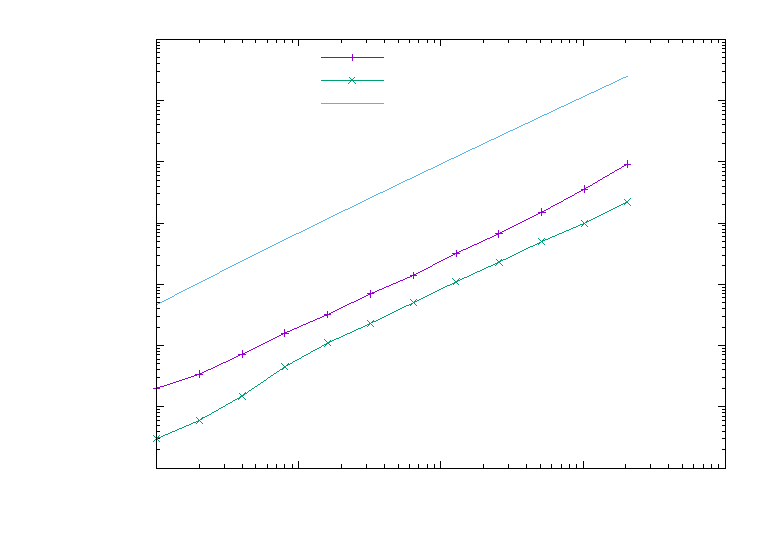
\includegraphics[width={360.00bp},height={252.00bp}]{disp}}%
    \gplfronttext
  \end{picture}%
\endgroup
}
    \caption{Visualization of sorting of LinkedList and Array using quicksort}   
    \label{tab:figure1} 
    
    \end{figure}
\FloatBarrier{\noindent}
The quicksort algorithm should usually follow a $O(nlog(n))$ which both of the algorithms seem to do according to the graph, even though the numbers for the algorithms are 
different they still have the same $O()$ function as they both increase in the same way compared to the previous amount of elements. 
\end{document}
